%!TEX ROOT=radek-novotny-bp-2017.tex
\chapter{Podklady}
V této kapitole jsou popsány mapové podklady využívané při výpočtu 
faktorů pro USLE. V České republice se jedná zejména o vrstvy 
BPEJ~($K, G_P$), LPIS~($C$) a~DMT($LS$).
\section{BPEJ}
Prvním krokem k vytvoření systému hodnocení půdy BPEJ bylo v roce 1961
zahájení celosvětově ojedinělého Komplexního průzkumu půd(KPP), při
kterém bylo odebráno okolo 700~000~ půdních sond, ze kterých byly
zpracovány mapové podklady. Na základě nichž byl v roce 1971 začala
tvorba systému ocenění zemědělské půdy - proběhla tzv.~Bonitace
zemědělského půdního fondu.

Původní mapy 1~:~5000 byly zvektorizovány do bonitačního informačního
systému, který je průběžně aktualizován a zpřesňován. Přehled všech
informací o BPEJ je dostupný v eKatalogu BPEJ od
VÚMOP\cite{bpej_vumop}. Ke 3.4.2017 Státní pozemkový úřad uvolnil
celostátní databázi volně ke stažení ve formátu Esri Shapefile\cite{spucr}.
\begin{figure}[H]
    \centering
    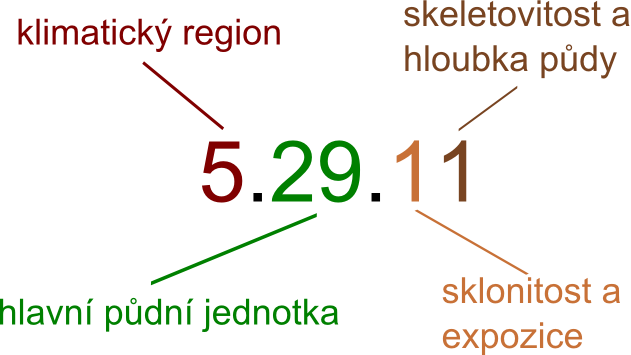
\includegraphics[scale=0.5]{./pictures/Struktura_BPEJ.png}
      \caption[Struktura kódu BPEJ]{Struktura kódu BPEJ, zdroj:
        VÚMOP\cite{bpej_vumop}}
      \label{fig:struktura_bpej}
\end{figure}
Bonitovaná půdně ekologická jednotka je vyjádřena pětimístným kódem ve
formátu - X.XX.XX. Kdy první číslice určuje příslušící klimatický
region(0-9). Druhá a třetí zařazuje půdu do hlavní půdní
jednotky(HPJ)(01-78), pomocí které je ve většině případů možné určit K
faktor~(viz. tab.\ref{hpj_k}). Čtvrtá číslice vymezuje kombinaci
sklonitosti a expozice svahu ke světovým stranám(0-9). Pátá číslice
určuje kombinaci skeletovitosti půdního profilu s hloubkou půdy(0-9),
tato číslice je využívána pro získání hloubky půdy při určení
$G_P$.\cite{Novotny2013}
\section{LPIS}
\begin{figure}[H]
    \centering 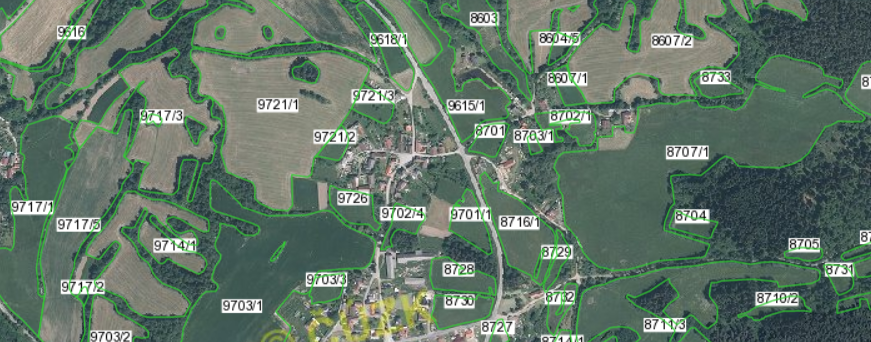
\includegraphics[scale=0.7]{./pictures/lpis.png}
      \caption[Ukázka GIS online aplikace Registr půd]{Ukázka online
        GIS aplikace Registr půd, zdroj: Registr půd\cite{lpis}}
      \label{fig:lpis}
\end{figure}
V roce 1999 se Česká republika zavázala vybudovat do vstupu do EU
systém evidence půdy, který bude založený na uživatelských
vztazích. Jelikož takový systém v ČR do té doby nebyl, tak první verze
z roku 2002 vznikla zakreslením půdních bloků z leteckých snímků do
offline geografického informačního systému, tyto bloky byly následně
schváleny příslušnými uživateli půdy. Toto první řešení bylo v roce
2004 nahrazeno online aplikací Registr půdy\cite{lpis}, která
usnadnila přístup k materiálům LPIS. Ty lze z Registru půdy exportovat
pro vybrané území.\cite{lpis}

Při výpočtu USLE se LPIS využívá k rozdělení na jednotlivé erozně
uzavřené celky(EUC) neboli pozemky, na kterých je eroze počítána. Dále
může být využito rozdělení pozemků dle kultur, pomocí kterého je možné
určit zakládní C faktor a~stanovit pozemky s ornou půdou, pro které je
třeba zjistit pěstované plodiny.\cite{Novotny2014}
\begin{table}[!h]
\begin{center}
\catcode`\-=12
    \noindent\begin{tabular}{|*{3}{c|}} \hline \bf Kód & \bf Kultura &
    \bf C faktor\\ \hline R & orná půda & dle pěstované
    plodiny\\ \hline C & chmelnice & 0,8\\ \hline V & vinice &
    0,8\\ \hline S & ovocný sad & 0,45\\ \hline T & travní porost &
    0,005\\ \hline L & zalesněno & 0,003-0,009\\ \hline O & jiná
    kultura & nutno určit kulturu\\ \hline
    \end{tabular}\\
  \caption[Rozdělení kultur na zemědělské půdě dle LPIS]{Rozdělení
    kultur na zemědělské půdě dle LPIS\cite{lpis} s C faktory
    dle\cite{janecek2012}.}
  \label{tabulka_c_typ}
\end{center}
\end{table}
\FloatBarrier
\section{DMT}
%%% ML: nejaky obrazek/screenshot?
%%% RN: Idealne bych chtel vlozit porovnani 4G/5G, zatim jsem
% nenasel nic vhodneho.
%%% ML: neco jako
%%% http://freegis.fsv.cvut.cz/gwiki/%C4%8C%C3%9AZK_DMT/DMP anebo http://training.gismentors.eu/grass-gis-pokrocily/lidar/dmr-dmp-cuzk.html ?
Pro výpočet LS faktoru se v ČR při využití GIS používají především
digitální model reliéfu vytvořenými ČÚZK\cite{cuzk}. Výpočty nad
DMR~4G jsou rychlejší díky pravidelné mřížce, zatímco výpočty nad
DMR~5G poskytují přesnější model terénu.
\subsection{DMR 4G}
%%% ML: Zbytecne dlouha veta
%%% RN: Rozdelil jsem ji na dve
Digitální model reliéfu České republiky 4.~generace~(DMR~4G)
vznikl leteckým laserovým skenováním v letech 2009 až 2013. DMR~4G 
zobrazuje přirozený nebo lidskou činností upravený zemský povrch v 
pravidelné síti 5~x~5~m, která je tvořena body s~určenou nadmořskou
výškou~(Bpv). Pro tento model byla vypočtena úplná střední chyba výšky
0,3~m v odkrytém terénu a 1~m v zalesněném terénu.
\subsection{DMR 5G}
Pro vytvoření páté generace digitálního modelu terénu byla použita
stejná data jako pro čtvrtou generaci. DMR~5G se tedy od předchozího
DMR~4G liší především použitím nepravidelné trojúhelníkové bodové
sítě~(TIN). Tím bylo dosaženo nižší úplné střední chyby výšky a to
0,18~m v odkrytém terénu a 0,3~m v zalesněném terénu.
